\documentclass[aspectratio=169,11pt]{beamer}

\usetheme{Madrid}
\usecolortheme{default}
\usefonttheme{professionalfonts}
\setbeamertemplate{navigation symbols}{}
\setbeamertemplate{footline}[frame number]

\usepackage{amsmath, amssymb, booktabs, graphicx}
\graphicspath{{../../assets/figures/}{assets/figures/}}

\title{Trade, Offshoring, and Labor Market Adjustment}
\subtitle{Labor II --- Week 12}
\author{Teaching deck draft}
\date{}

\begin{document}

\begin{frame}
  \titlepage
\end{frame}

\begin{frame}{Central question and week repositioning}
\begin{itemize}
    \item How do trade and offshoring shocks transmit through workers, firms, sectors, and places?
    \item Week 12 is a labor-market adjustment lecture, not a generic trade lecture.
    \item The same trade shock can move wages, employment, unemployment, nonparticipation, sector shares, and welfare on different horizons.
\end{itemize}
\end{frame}

\begin{frame}{Week 11 to Week 12 bridge}
\begin{itemize}
    \item Week 11: shocks began inside production through task change, automation, and organizational redesign.
    \item Week 12: shocks begin through global integration, relative prices, and the location of production.
    \item Both weeks study adjustment, but trade must keep import competition, export exposure, offshoring, and structural change separate.
\end{itemize}
\end{frame}

\begin{frame}{Why trade is not just a demand shock}
\begin{itemize}
    \item Import competition can contract exposed sectors and places.
    \item Export access can expand labor demand and wage opportunities.
    \item Offshoring and imported intermediates can reorganize tasks inside firms.
    \item Structural change can shift employment from manufacturing to services.
    \item Mobility frictions determine whether workers, firms, and places adjust together.
\end{itemize}
\end{frame}

\begin{frame}{Trade channel map}
\begin{center}
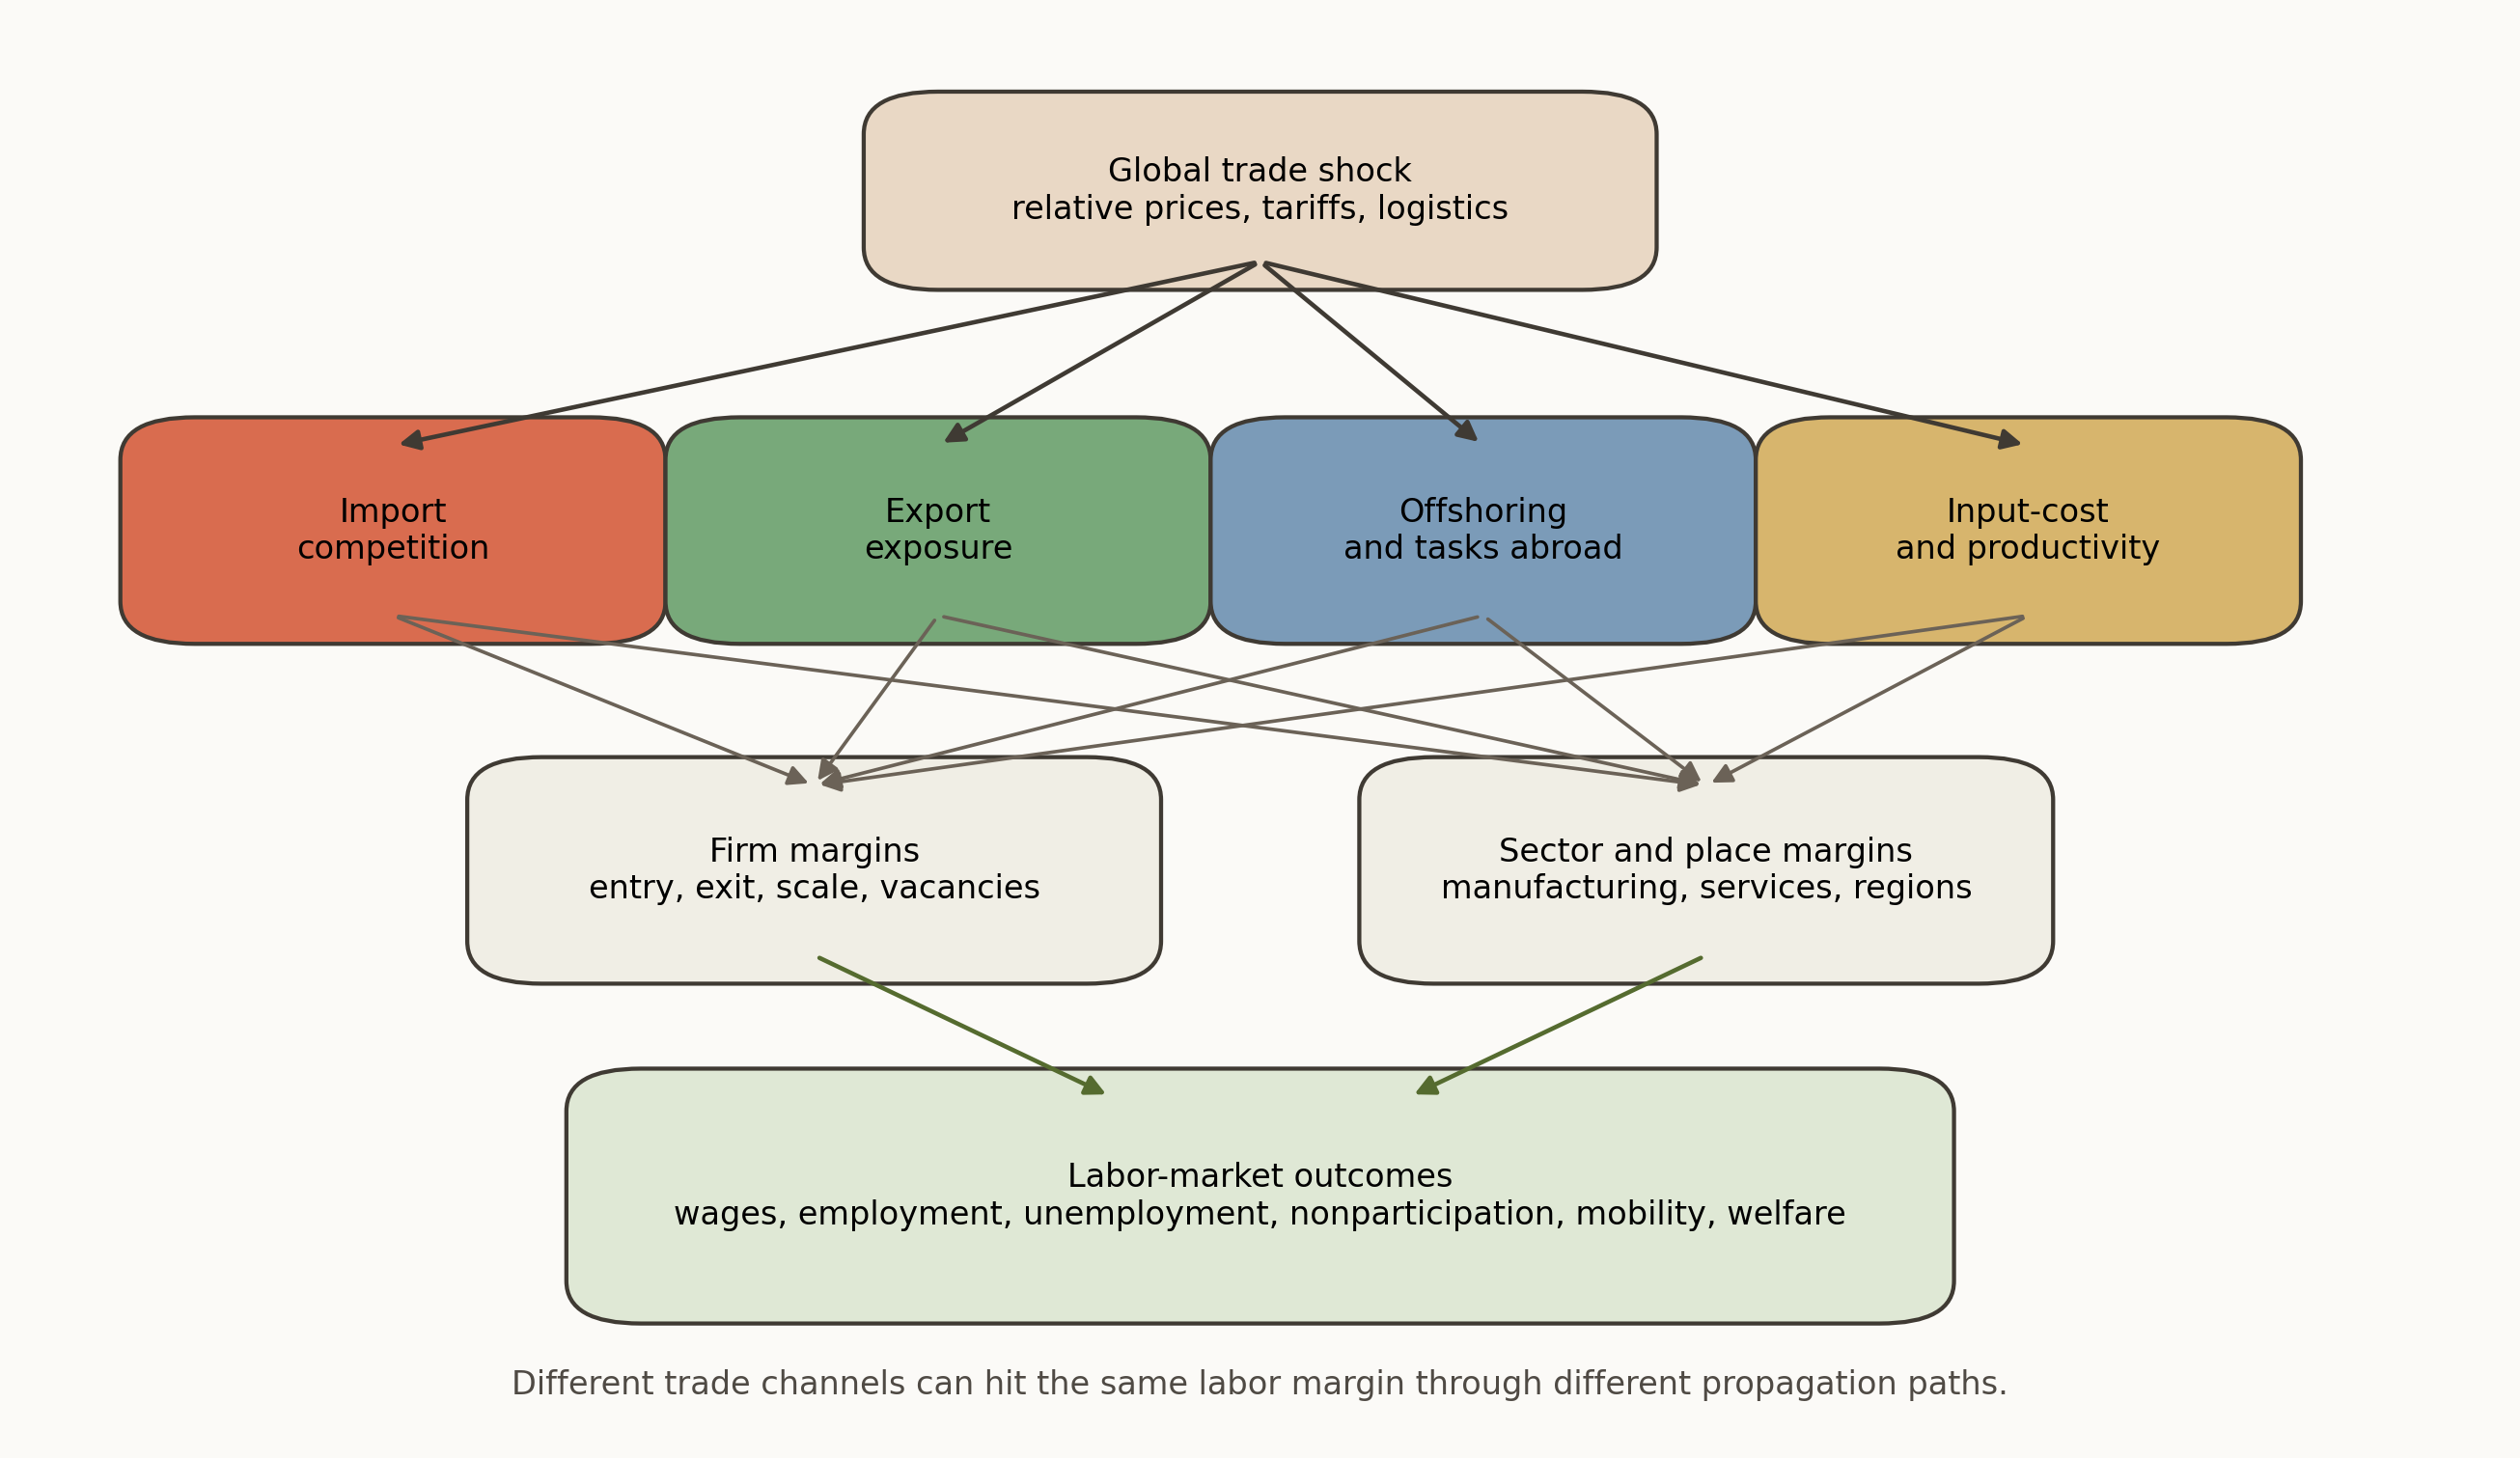
\includegraphics[height=0.73\textheight]{12-trade-channels-framework.png}
\end{center}
\end{frame}

\begin{frame}{One local labor-market exposure object}
\[
\text{Exposure}_r = \sum_s \omega_{rs,0}\,\Delta \text{TradeShock}_s
\]

\begin{itemize}
    \item Baseline sector shares map a sectoral trade shock into local exposure.
    \item The treatment object changes when the unit is a worker, firm, or place.
    \item Exposure is not yet a welfare object; it is an incidence object.
\end{itemize}
\end{frame}

\begin{frame}{What the reduced-form outcome equation identifies}
\[
\Delta y_r = \beta \,\text{Exposure}_r + X_r'\Gamma + \varepsilon_r
\]

\begin{itemize}
    \item The observed margin might be employment, wages, unemployment, nonparticipation, or sector shares.
    \item Local designs are strongest on place-level incidence.
    \item Migration, worker transitions, and aggregate price adjustment remain partly offstage.
\end{itemize}
\end{frame}

\begin{frame}{Import competition, export exposure, and offshoring}
\begin{itemize}
    \item Import competition: foreign supply shock in competing sectors.
    \item Export exposure: market-access gains and local expansion.
    \item Offshoring: relocation of tasks or intermediate stages abroad.
    \item Input-cost channel: cheaper intermediates raise productivity for some firms.
    \item Structural-change channel: trade shifts sector composition and service demand.
\end{itemize}
\end{frame}

\begin{frame}{China syndrome and local U.S. adjustment}
\begin{itemize}
    \item Autor-Dorn-Hanson: commuting-zone exposure to Chinese import growth.
    \item Unit: place. Margin: employment, wages, unemployment, nonparticipation.
    \item Core result: more exposed places saw larger manufacturing decline and weaker labor outcomes.
    \item Interpretation: identifies place incidence, not full worker welfare or aggregate gains from trade.
\end{itemize}
\end{frame}

\begin{frame}{Policy exposure and manufacturing decline}
\begin{itemize}
    \item Pierce-Schott links manufacturing decline to the policy environment around China trade integration.
    \item Unit: industry. Margin: manufacturing employment decline.
    \item Lesson: trade shocks also operate through uncertainty resolution, firm exit, and industry restructuring.
\end{itemize}
\end{frame}

\begin{frame}{Dynamic adjustment needs a horizon object}
\[
y_{rt+h} - y_{rt-1}
=
\sum_{h \in \mathcal{H}} \beta_h \,\text{Exposure}_{r}
+ X_{rt}'\Gamma_h + \varepsilon_{rt+h}
\]

\begin{itemize}
    \item Short-run displacement and long-run adjustment are different empirical objects.
    \item Event-time responses discipline claims about persistence and recovery.
    \item Regional recovery need not imply that initially displaced workers are whole again.
\end{itemize}
\end{frame}

\begin{frame}{Brazil and dynamic regional adjustment}
\begin{itemize}
    \item Dix-Carneiro-Kovak: regional exposure to tariff reform over long horizons.
    \item Unit: region over time. Margins: earnings, employment structure, persistent adjustment.
    \item Main lesson: regional labor markets adjust slowly, so early losses and long-run outcomes can differ sharply.
\end{itemize}
\end{frame}

\begin{frame}{Worker versus place adjustment}
\begin{center}
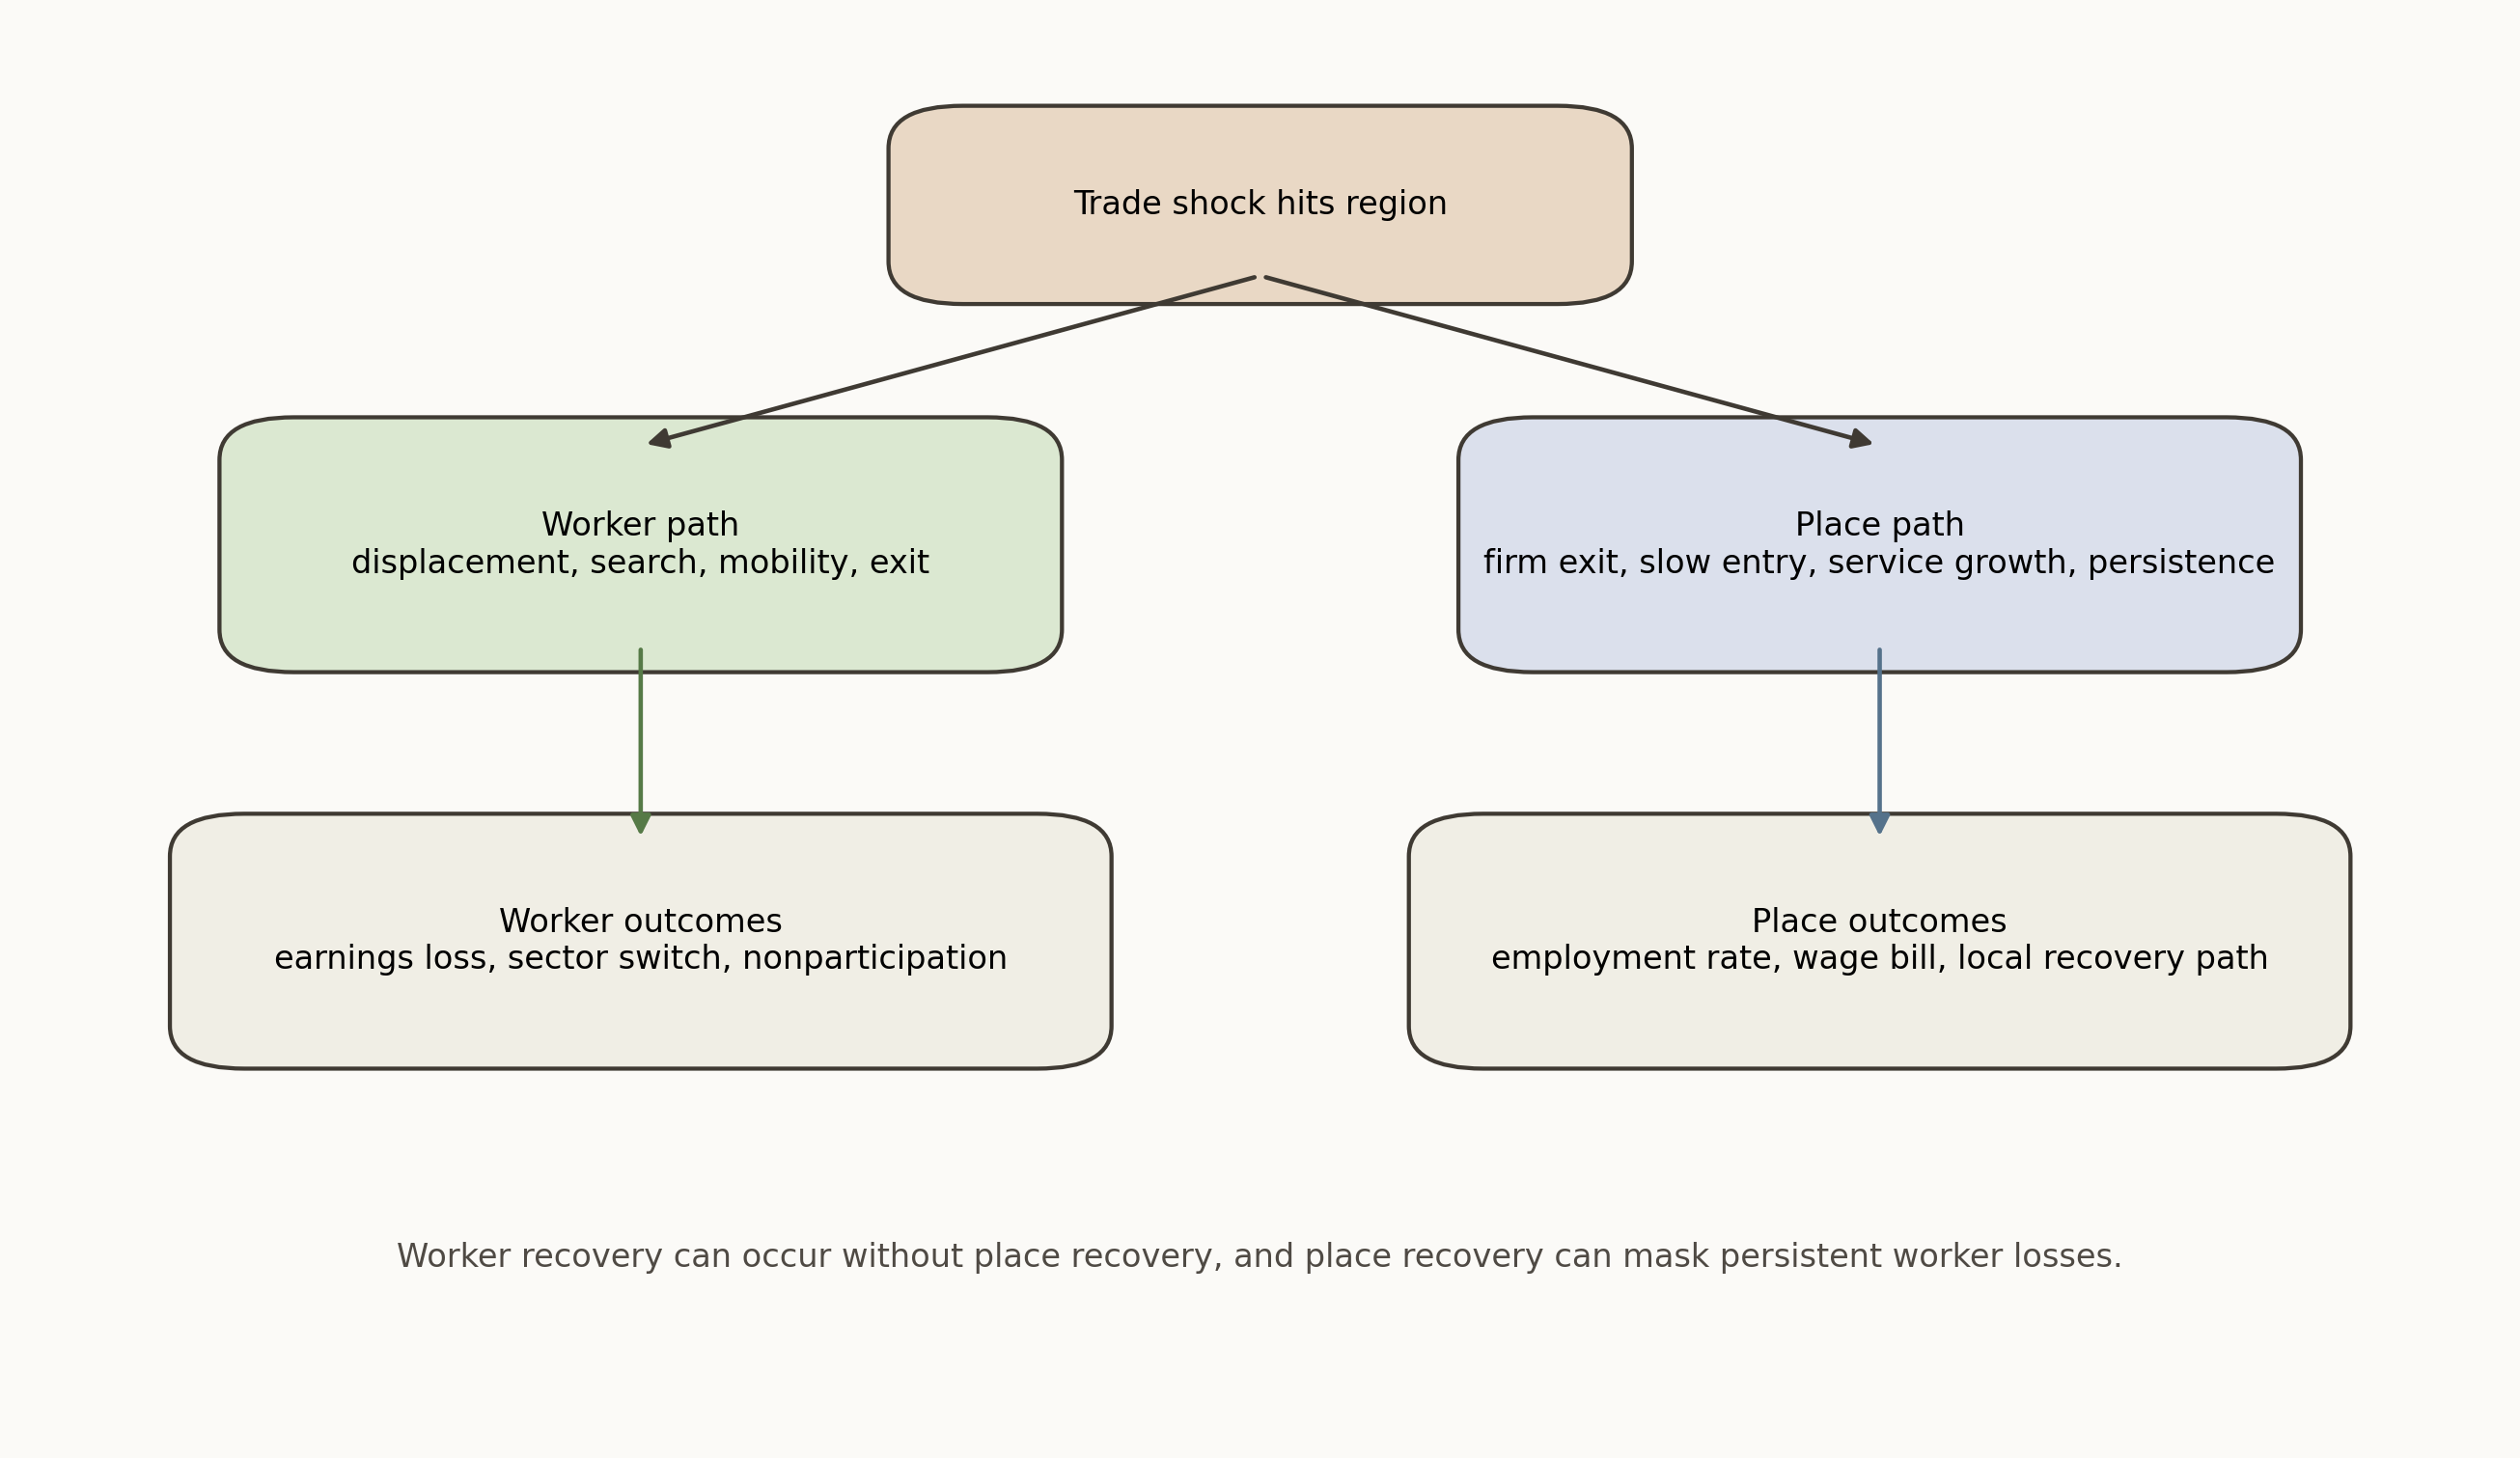
\includegraphics[height=0.72\textheight]{12-trade-adjustment-worker-vs-place.png}
\end{center}
\end{frame}

\begin{frame}{Trade-induced structural change}
\[
\Delta \log \frac{L_M}{L_S}
=
\eta_p \,\Delta \log \frac{P_M}{P_S}
+
\eta_y \,\Delta \log Y
+
\eta_a \,\Delta \log \frac{A_M}{A_S}
\]

\begin{itemize}
    \item Manufacturing-to-service transition can come from relative prices, expenditure shifts, and productivity differences.
    \item Sectoral reallocation is not enough; the lecture must ask who actually moves.
\end{itemize}
\end{frame}

\begin{frame}{Germany, structural change, and service transitions}
\begin{itemize}
    \item Dauth-Findeisen-Suedekum: German exposure to Eastern Europe and China.
    \item Unit: workers and regions. Margins: manufacturing decline, service growth, transition margins.
    \item Key lesson: observed service expansion is not simply incumbent manufacturing workers gliding into service jobs.
\end{itemize}
\end{frame}

\begin{frame}{Manufacturing-to-service transitions}
\begin{center}
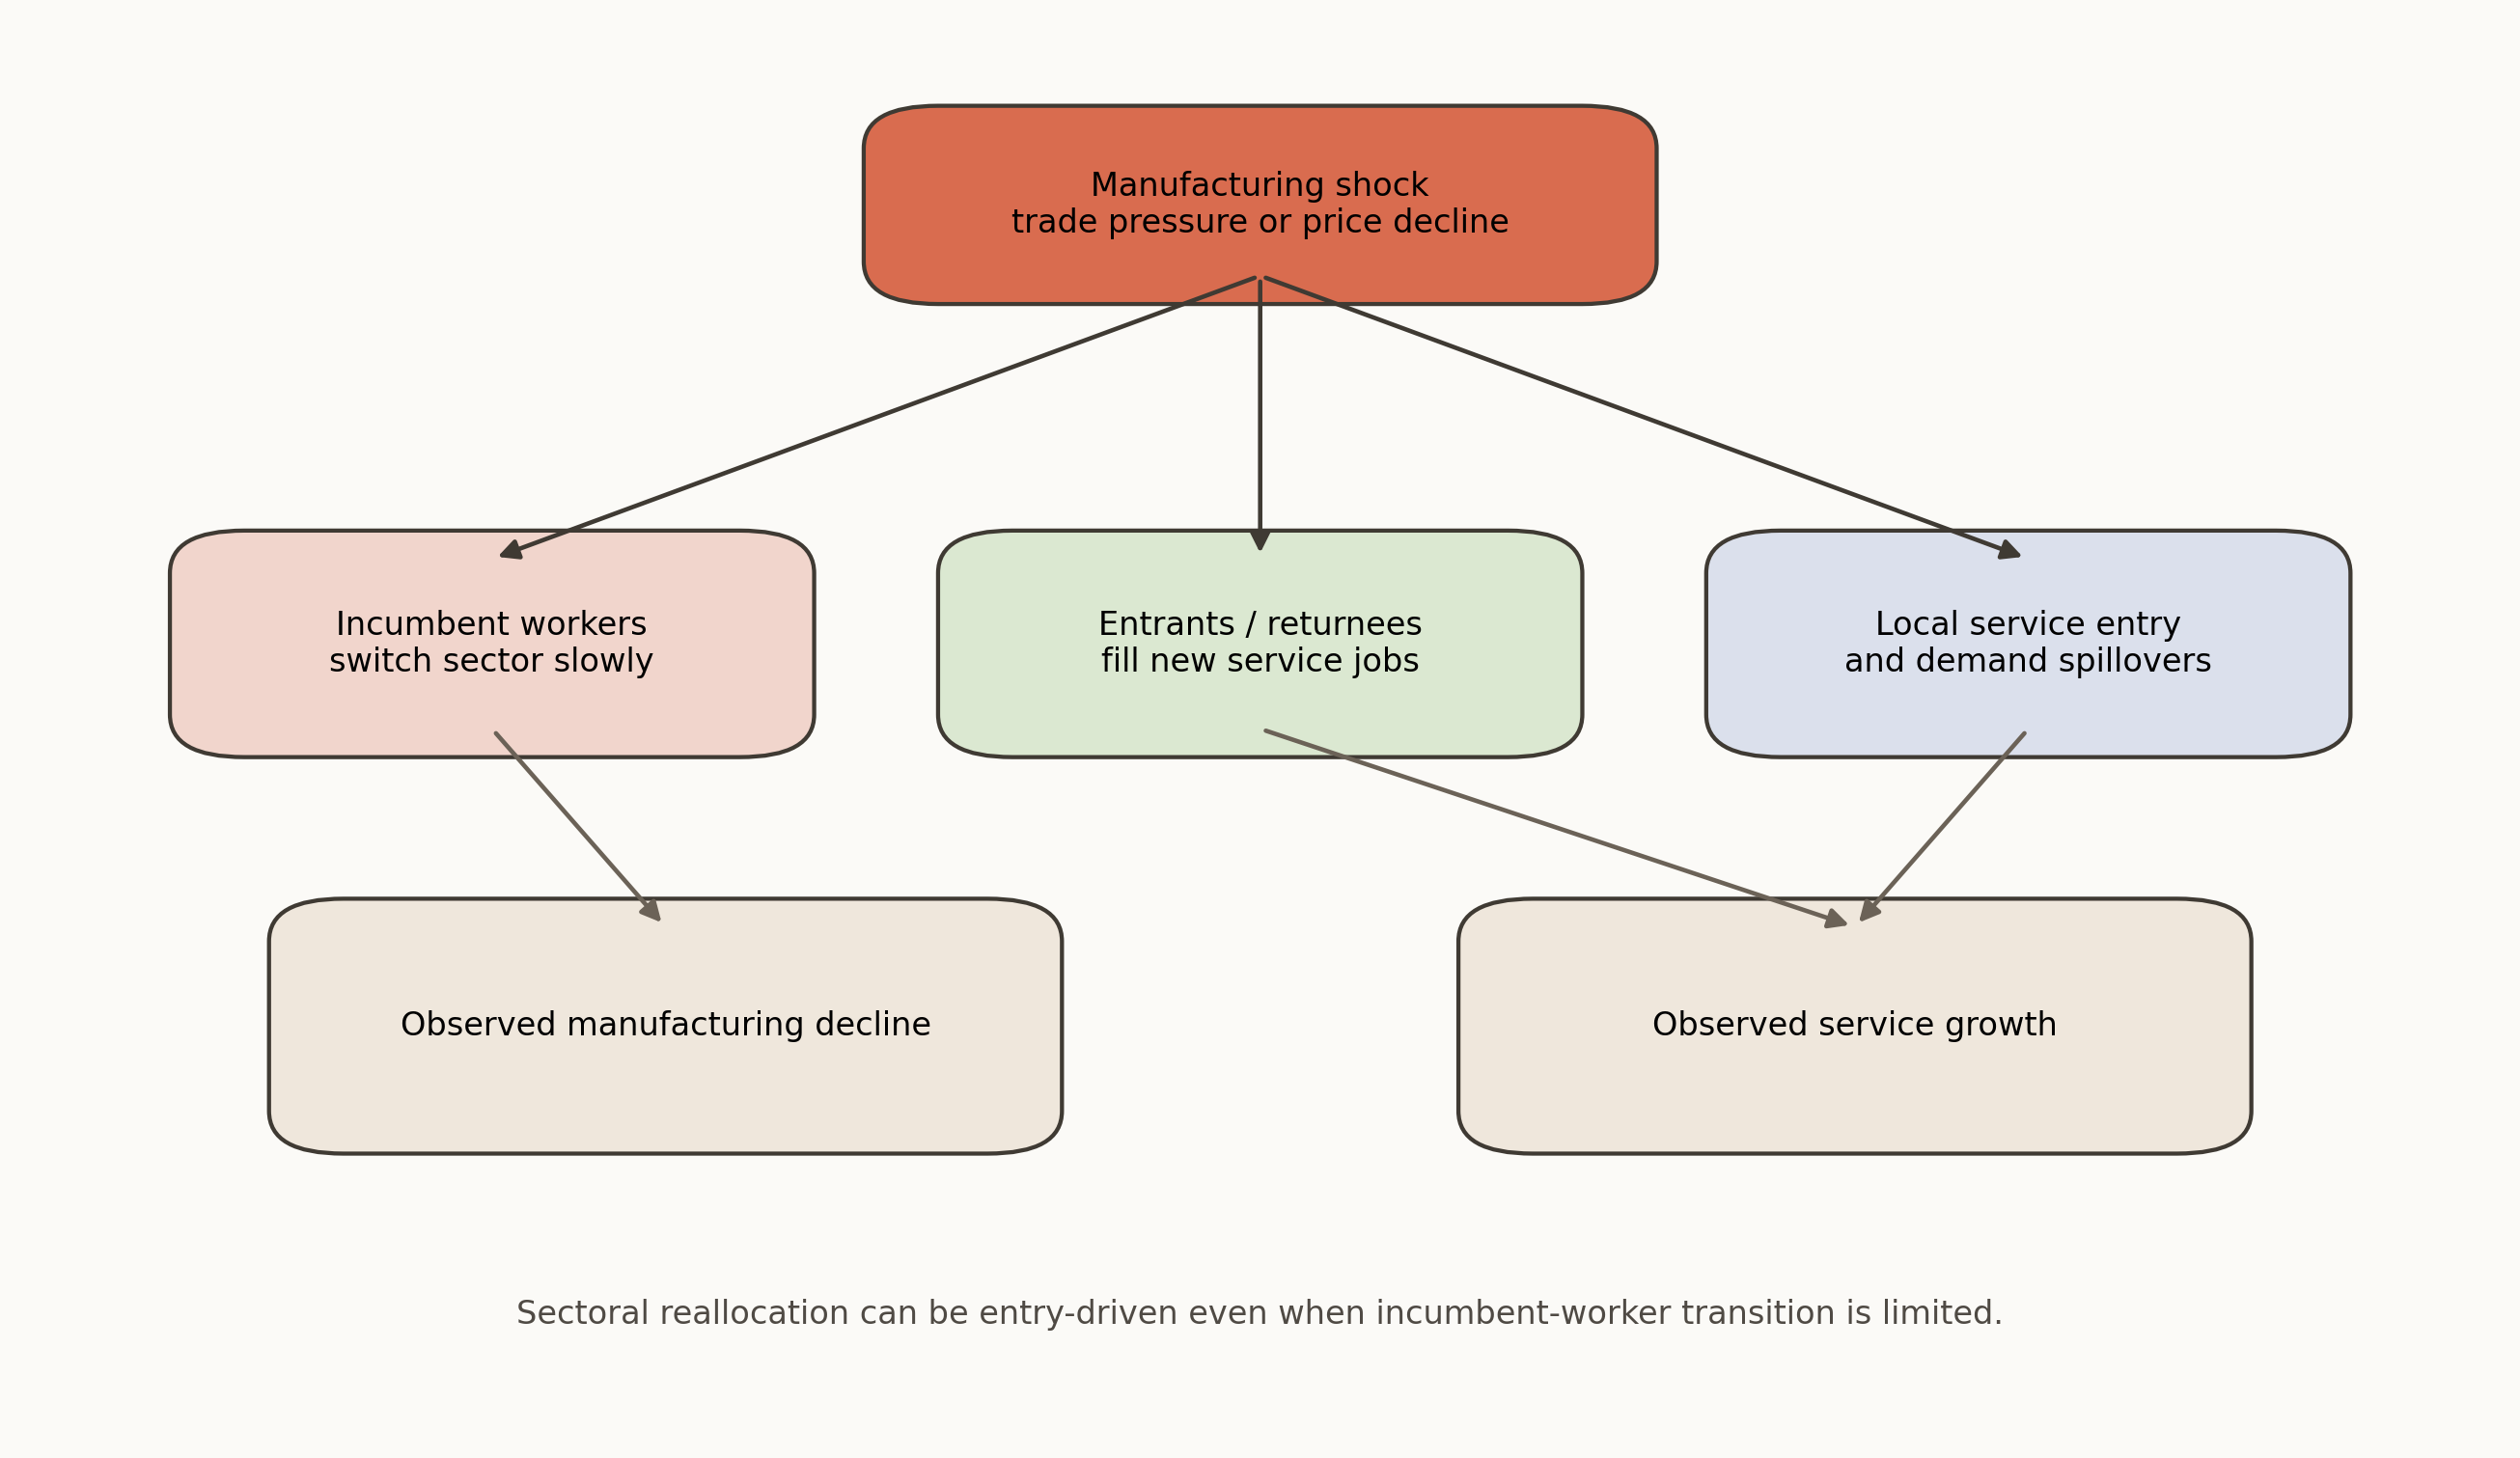
\includegraphics[height=0.72\textheight]{12-trade-structural-change-transitions.png}
\end{center}
\end{frame}

\begin{frame}{Offshoring and services trade as a distinct channel}
\begin{itemize}
    \item Feenstra-Hanson: outsourcing changes within-firm organization and relative demand.
    \item Offshoring is not the same object as final-goods import competition.
    \item Imported intermediates, fragmented tasks, and services trade can alter skill demand even when local import exposure is modest.
\end{itemize}
\end{frame}

\begin{frame}{Worker losses, place losses, and welfare}
\[
\Delta W =
\sum_i \pi_i \,\Delta \text{RealIncome}_i
- \sum_i \text{TransitionCost}_i
- \sum_r \text{PlaceAdjustmentCost}_r
\]

\begin{itemize}
    \item Worker losses, place losses, and aggregate gains are distinct objects.
    \item Local labor-market estimates are central for incidence but insufficient for welfare.
    \item Structured frameworks are needed for policy counterfactuals.
\end{itemize}
\end{frame}

\begin{frame}{Trade, welfare, and reallocation}
\begin{center}
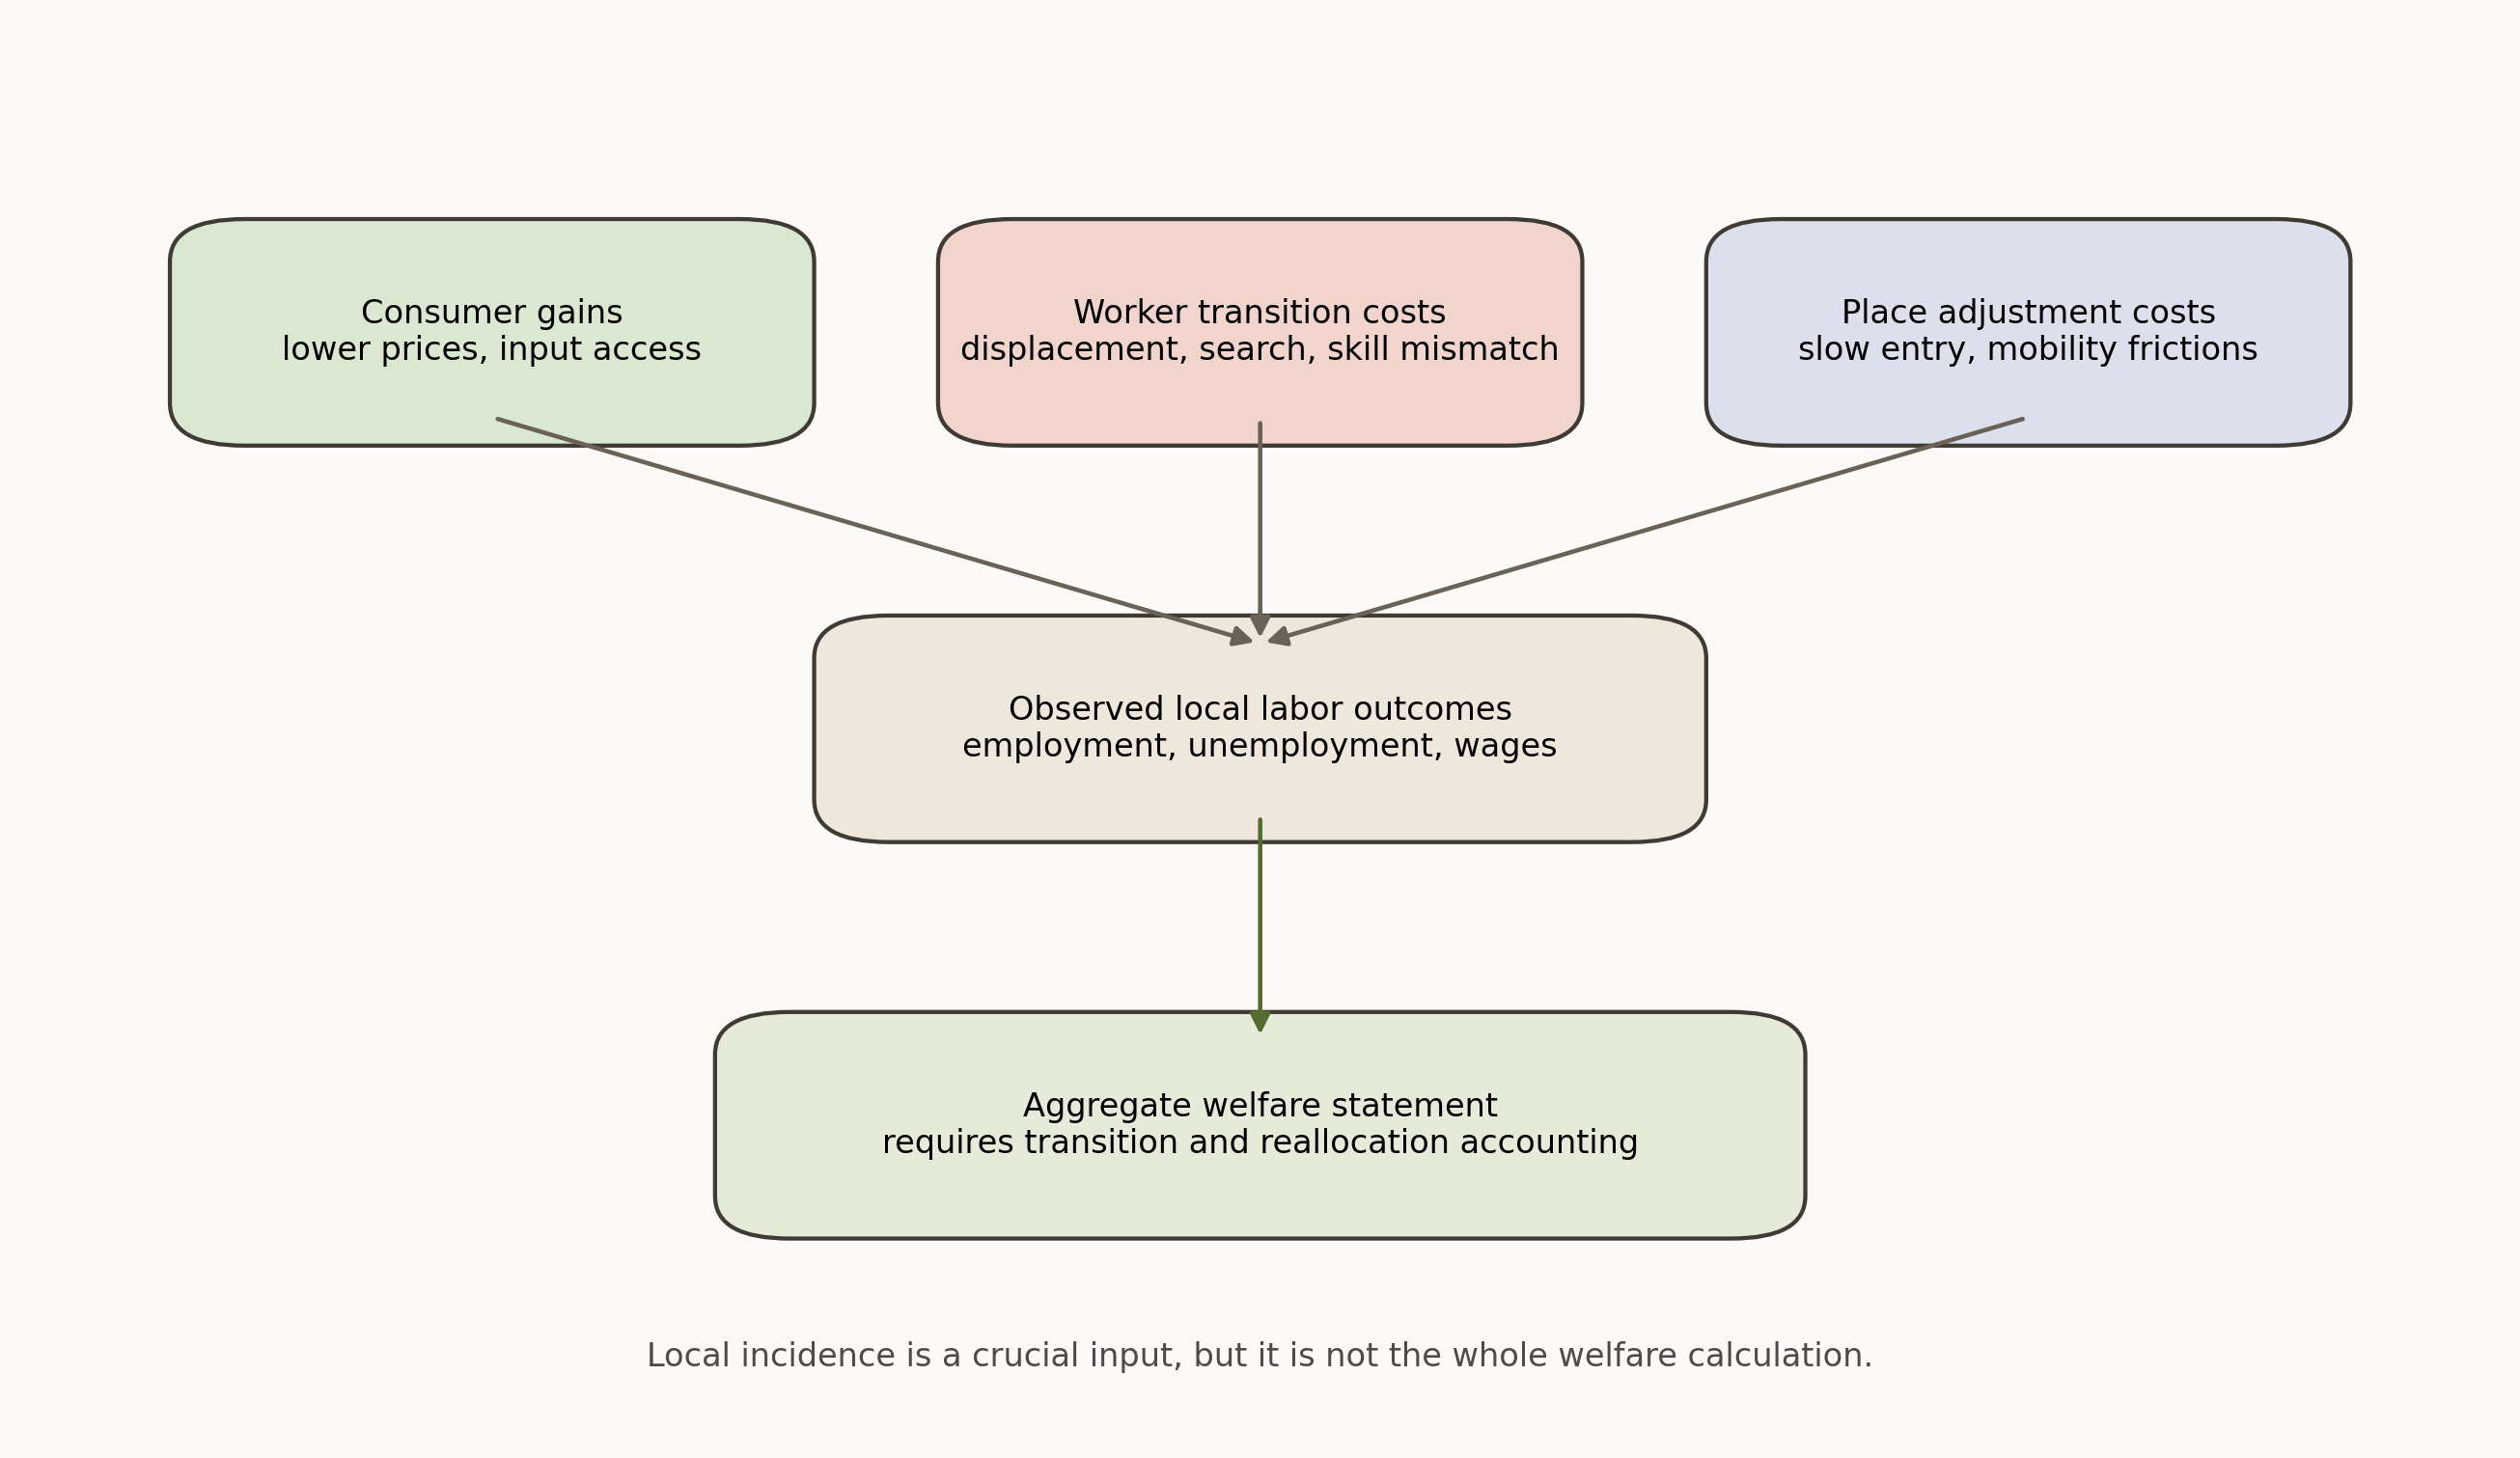
\includegraphics[height=0.72\textheight]{12-trade-welfare-and-reallocation.png}
\end{center}
\end{frame}

\begin{frame}{Structured equilibrium frameworks}
\begin{itemize}
    \item Kim-Vogel: trade shocks with unemployment, nonparticipation, and adjustment frictions.
    \item Caliendo-Dvorkin-Parro: dynamic general equilibrium analysis of the China trade shock.
    \item What structure adds: transition paths, worker reallocation, consumer gains, and welfare accounting.
\end{itemize}
\end{frame}

\begin{frame}{Global evidence and frontier directions}
\begin{center}
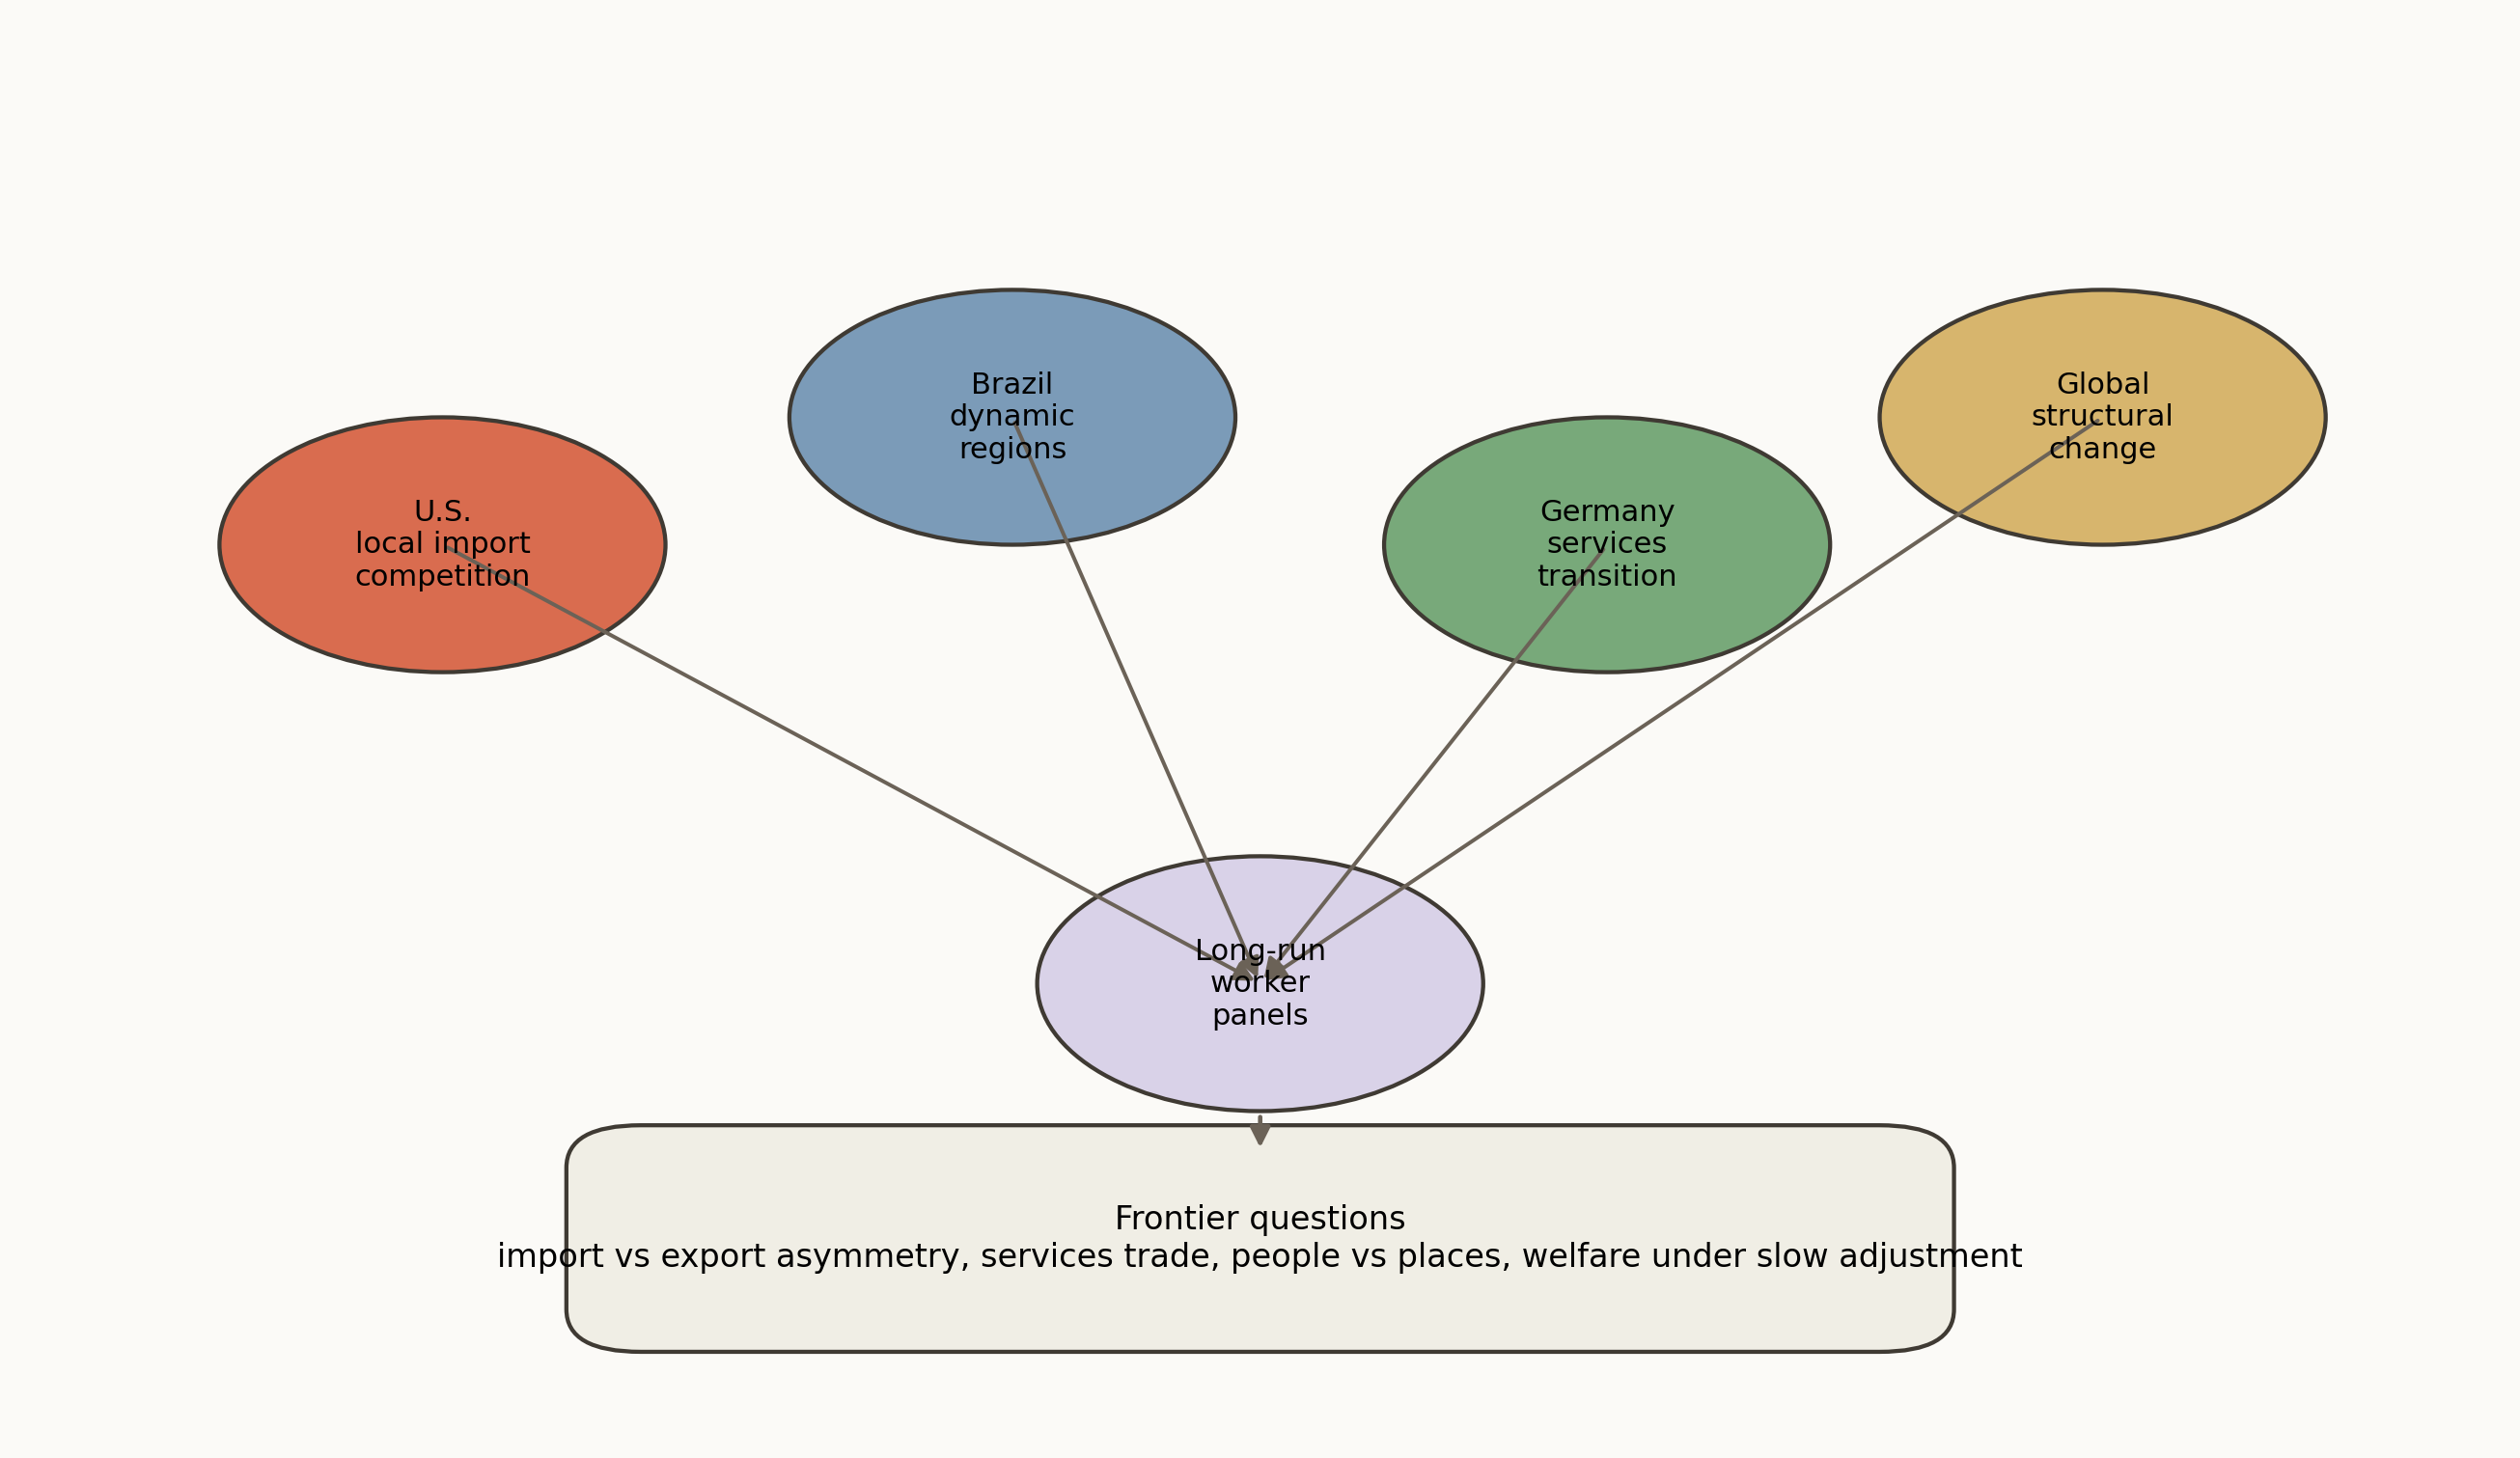
\includegraphics[height=0.72\textheight]{12-trade-global-evidence-and-frontiers.png}
\end{center}
\end{frame}

\begin{frame}{New research directions}
\begin{itemize}
    \item Worker panels versus place panels
    \item Import versus export asymmetry
    \item Services trade and white-collar offshoring
    \item Structural change into services and the role of entrants
    \item Trade, labor-market power, and local concentration
    \item Welfare and policy evaluation under slow adjustment
\end{itemize}
\end{frame}

\begin{frame}{Bridge to Week 13 synthesis}
\begin{itemize}
    \item Week 11 and Week 12 together complete the major shock-and-adjustment block of Labor II.
    \item Week 13 will ask how firms, frictions, institutions, and shocks fit into one research design toolkit.
    \item The synthesis question is no longer whether trade matters, but which object, margin, and horizon a given design actually identifies.
\end{itemize}
\end{frame}

\begin{frame}{Takeaways}
\begin{itemize}
    \item Trade affects labor markets through several distinct channels, not just import competition.
    \item Local exposure designs identify place incidence, not full worker welfare.
    \item Dynamic evidence and structural change evidence are essential for understanding persistence.
    \item Worker adjustment, place adjustment, and aggregate welfare should never be conflated.
\end{itemize}
\end{frame}

\appendix

\begin{frame}{Appendix: Week 12 lab bridge}
\begin{itemize}
    \item Reproduce: a bounded China-syndrome-style commuting-zone exposure exercise.
    \item Diagnose: identify the channel, unit, margin, and hidden adjustment margin.
    \item Transfer: carry the same exposure logic into a synthetic structural-change setting.
    \item Challenge extension: compare short-run place effects to dynamic regional adjustment.
\end{itemize}
\end{frame}

\end{document}
